\section{Introduction}
\begin{frame}{What is Computer Science?}
    \begin{itemize}
        \item Computer Science is not merely the study of computers.
        \item Computers are tools that aid in problem-solving.
        \item The focus is on problems, problem-solving, and algorithmic solutions.
    \end{itemize}
\end{frame}

\begin{frame}{The Role of Algorithms}
    \begin{itemize}
        \item An algorithm is a step-by-step set of instructions to solve a problem.
        \item Some problems may not have a solution.
        \item Computer Science studies both solvable and unsolvable problems.
    \end{itemize}
\end{frame}

\begin{frame}{Computability in Computer Science}
    \begin{itemize}
        \item A problem is \textbf{computable} if an algorithm exists to solve it.
        \item Computer Science studies both computable and non-computable problems.
        \item Solutions are independent of the machine used.
    \end{itemize}
\end{frame}

\begin{frame}{Abstraction in Computer Science}
    \begin{itemize}
        \item Abstraction helps separate the logical and physical perspectives.
        \item Example: Driving a car.
        \item Users interact with the interface without needing to understand the mechanics.
    \end{itemize}
\end{frame}

\begin{frame}[fragile]{Procedural Abstraction}
    \begin{itemize}
        \item Users (clients) do not need to know implementation details.
        \item The interface provides a way to interact with complex implementations.
        \item Example: Python's \texttt{math} module.
    \end{itemize}

    \vspace{0.5cm} % Adds space for better readability

    
    \begin{lstlisting}[language=Python]
import math
math.sqrt(16)
    \end{lstlisting}

    \vspace{0.5cm} % Adds space before continuing the list

    \begin{itemize}
        \item We do not need to know how \texttt{sqrt} is implemented.
        \item We only need to know its name and how to use it.
    \end{itemize}
\end{frame}

\begin{frame}{Programming and Algorithms}
    \begin{itemize}
        \item Programming is encoding an algorithm into a notation (programming language) for computer execution
        \item Without an algorithm, there can be no program
        \item Computer science is not just programming, but programming is an essential part
        \item Programming creates representations of our solutions
    \end{itemize}
\end{frame}

\begin{frame}{From Algorithms to Programs}
    \begin{itemize}
        \item Algorithms describe solutions in terms of:
        \begin{itemize}
            \item Data needed to represent the problem instance
            \item Steps necessary to produce the intended result
        \end{itemize}
        \item Programming languages must provide notation for both process and data
        \item Languages provide control constructs and data types
    \end{itemize}
\end{frame}

\begin{frame}{Control Constructs}
    \begin{itemize}
        \item Control constructs allow algorithmic steps to be represented unambiguously
        \item Minimum requirements for algorithm representation:
        \begin{itemize}
            \item Sequential processing
            \item Selection for decision-making
            \item Iteration for repetitive control
        \end{itemize}
        \item Any language with these basic statements can represent algorithms
    \end{itemize}
\end{frame}

\begin{frame}{Data Types}
    \begin{itemize}
        \item All data in computers are strings of binary digits
        \item Data types provide interpretation for binary data
        \item Built-in/primitive data types are building blocks for algorithm development
        \item Example: Integer data type
        \begin{itemize}
            \item Binary digits interpreted as familiar numbers (23, 654, -19)
            \item Supports operations like addition, subtraction, multiplication
        \end{itemize}
    \end{itemize}
\end{frame}

\begin{frame}{Complexity Challenges}
    \begin{itemize}
        \item Problems and solutions are often very complex
        \item Simple language-provided constructs and data types:
        \begin{itemize}
            \item Are sufficient to represent complex solutions
            \item But can be at a disadvantage during problem-solving
        \end{itemize}
        \item Higher-level abstractions help manage this complexity
    \end{itemize}
\end{frame}

\begin{frame}{Abstraction in Problem-Solving}
    \begin{itemize}
        \item Computer scientists use abstractions to focus on the ``big picture''
        \item Creating models of the problem domain enables:
        \begin{itemize}
            \item More efficient problem-solving process
            \item More consistent description of data with respect to the problem
        \end{itemize}
        \item Abstractions allow us to ignore implementation details temporarily
    \end{itemize}
\end{frame}

\begin{frame}{Data Abstraction}
    \begin{itemize}
        \item Abstract Data Type (ADT): logical description of data and operations
        \item Focuses on \textit{what} the data represents, not \textit{how} it's constructed
        \item Creates encapsulation around data through information hiding
        \item Users interact with the interface only, not the implementation
    \end{itemize}
\end{frame}

\begin{frame}{ADT Implementation}
    \begin{itemize}
        \item Implementation of an ADT is called a data structure
        \item Data structure provides the physical view of the data
        \item Uses programming constructs and primitive data types
        \item Different implementations can satisfy the same ADT
        \item Choice of implementation affects efficiency
    \end{itemize}
\end{frame}

\begin{frame}{Python and High-Level Languages}
    \begin{itemize}
        \item Python is a \textbf{high-level programming language} (e.g., C++, PHP, Java).
        \item \textbf{High-level vs. Low-level languages:}
        \begin{itemize}
            \item High-level languages are easier to write, read, and debug.
            \item Low-level languages (machine/assembly) run directly on hardware.
            \item High-level programs need to be \textbf{processed} before execution.
        \end{itemize}
    \end{itemize}
\end{frame}

\begin{frame}{Advantages of High-Level Languages}
    \begin{itemize}
        \item \textbf{Easier} to program and debug.
        \item \textbf{More portable} – can run on different computers with minimal changes.
        \item \textbf{More readable} and maintainable.
    \end{itemize}
\end{frame}

\begin{frame}{Processing High-Level Languages}
    \begin{itemize}
        \item \textbf{Interpreters}: Execute code line by line.
        \item \textbf{Compilers}: Translate code into machine language before execution.
        \item Many modern languages use \textbf{both} methods (e.g., byte code + virtual machine).
    \end{itemize}
\end{frame}

\begin{frame}{Python Execution}
    \begin{itemize}
        \item Uses both \textbf{compilation (byte code)} and \textbf{interpretation (virtual machine)}.
        \item Mostly considered an \textbf{interpreted language}.
        \item Can be run in-browser for learning but also supports \textbf{local installation}.
    \end{itemize}
\end{frame}

\begin{frame}
    \begin{figure}
        \centering
        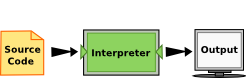
\includegraphics[width=0.8\textwidth]{pics/interpret.png}
        \caption{Python Execution}
        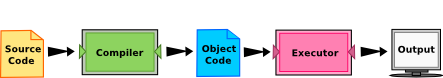
\includegraphics[width=0.8\textwidth]{pics/compile.png}
        \caption{Python Compilation}
    \end{figure}
\end{frame}